\documentclass[aspectratio=169]{beamer}

\usepackage{graphicx}
\usepackage{amsmath}

\title{Neural Network Integration into ODE Systems}
\author{Aksel Boukhalfa}
\date{July 2024}

\begin{document}

\begin{frame}
  \titlepage
\end{frame}

\begin{frame}
  \frametitle{Population Dynamics}

  \begin{itemize}   
    \item \text{Key Concepts}
      \begin{itemize}
        \item \textit{Exponential Growth:}
          \[
          \frac{dN}{dt} = rN
          \]
        \item \textit{Logistic Growth:}
          \[
          \frac{dN}{dt} = rN \left(1 - \frac{N}{K}\right)
          \]
      \end{itemize}

    \item \text{Key Factors}
      \begin{itemize}
        \item Birth Rate and Death Rate.
      \end{itemize}

    \item \text{Interaction with the Environment}
      \begin{itemize}
        \item Carrying Capacity (K).
        \item Density-Dependent and Density-Independent Factors.
      \end{itemize}

    \item \text{Types of Population Interactions}
      \begin{itemize}
        \item Predation, Competition, 
      \end{itemize}
    \item \text{Modeling Tools}
      \begin{itemize}
        \item Mathematical and Simulation Models.
      \end{itemize}
  \end{itemize}

\end{frame}


\begin{frame}
  \frametitle{Introduction}
  \begin{itemize}
    \item Overview of integrating neural networks into ODE systems.
    \item Objective: Visualize how neural network approximations affect ODE predictions.
    \item Methods: Use Julia for solving ODEs and training neural networks.
  \end{itemize}
\end{frame}

\begin{frame}
  \frametitle{Methodology }
  \begin{itemize}
    \item Define ODE system (Lotka-Volterra model).
    \item Generate noisy data and fit a neural network.
    \item Extend time span for prediction.
    \item Visualize network’s predictions integrated into the ODE system.
  \end{itemize}
\end{frame}

\begin{frame}
  \frametitle{Data Generation}
  \begin{itemize}
    \item Lotka-Volterra model equations:
    \[
    \frac{dx}{dt} = \alpha x - \beta xy
    \]
    \[
    \frac{dy}{dt} = \gamma xy - \delta y
    \]
    \item Experimental parameters and initial conditions.
  \end{itemize}
\end{frame}

\begin{frame}
  \frametitle{Noisy Data}
  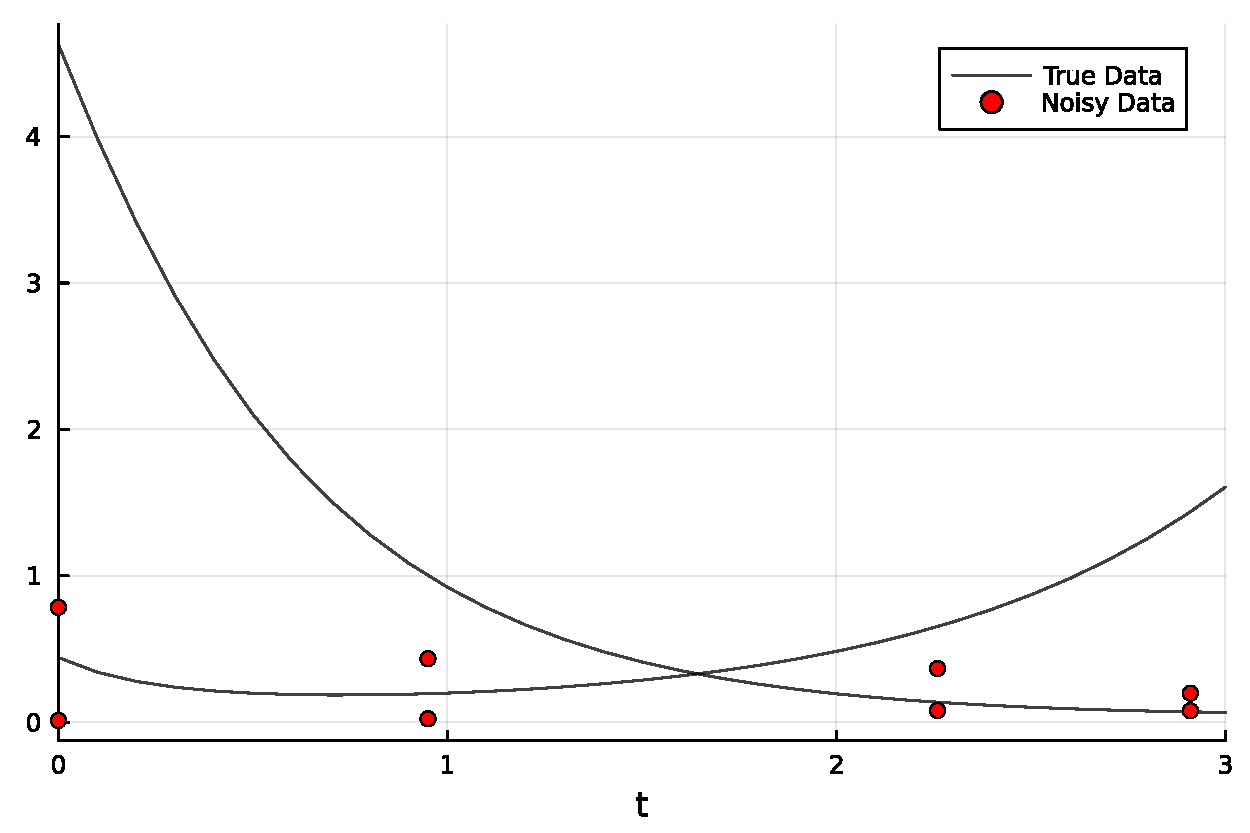
\includegraphics[width=12cm]{plots/Chemostat_noisydata.pdf}
\end{frame}

\begin{frame}
  \frametitle{NODE Approach}
  \begin{itemize}
    \item Network architecture: Multi-layer feedforward with RBF activation.
    \item Training process using ADAM and BFGS optimizers.
    \item Loss function and optimization.
  \end{itemize}
\end{frame}

\begin{frame}
  \frametitle{Network Architecture}

  \begin{figure}
    \centering
    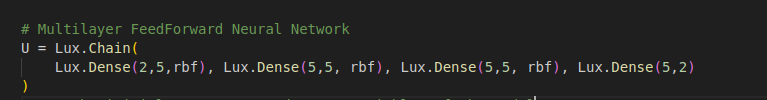
\includegraphics[width=1.0\textwidth]{plots/Screenshot from 2024-08-01 00-20-22.png}
    \caption{Neural Network Initialization}
    \vspace{1em} % Space between the images
    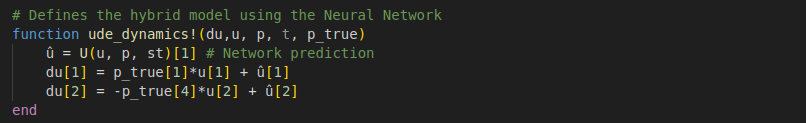
\includegraphics[width=1.0\textwidth]{plots/Screenshot from 2024-08-01 00-20-42.png}
    \caption{Integration into Differential Equation}
  \end{figure}

\end{frame}

\begin{frame}
  \frametitle{Training Loss}
  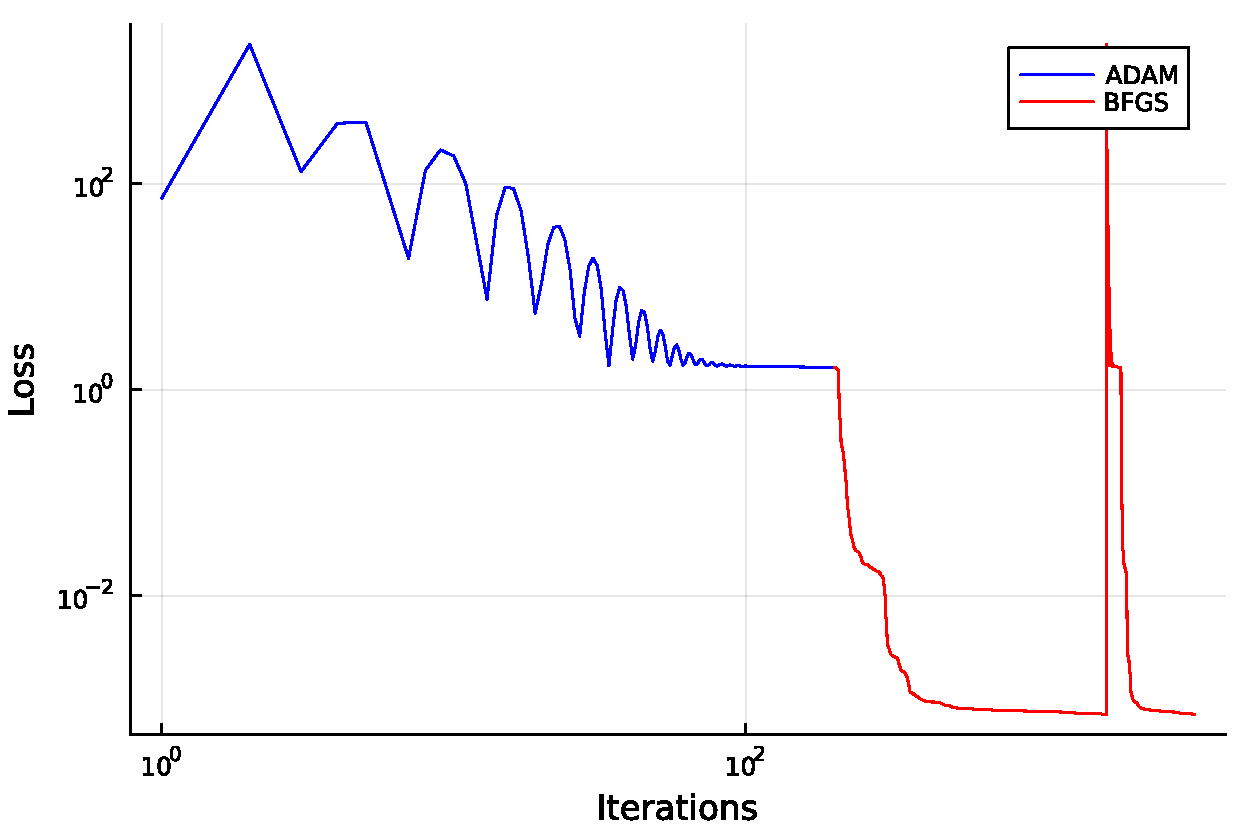
\includegraphics[width=12cm]{plots/Ideal_Data__losses.pdf}
\end{frame}

\begin{frame}
  \frametitle{Trajectory Reconstruction}
  \begin{itemize}
    \item Comparison of model predictions with true data.
  \end{itemize}
  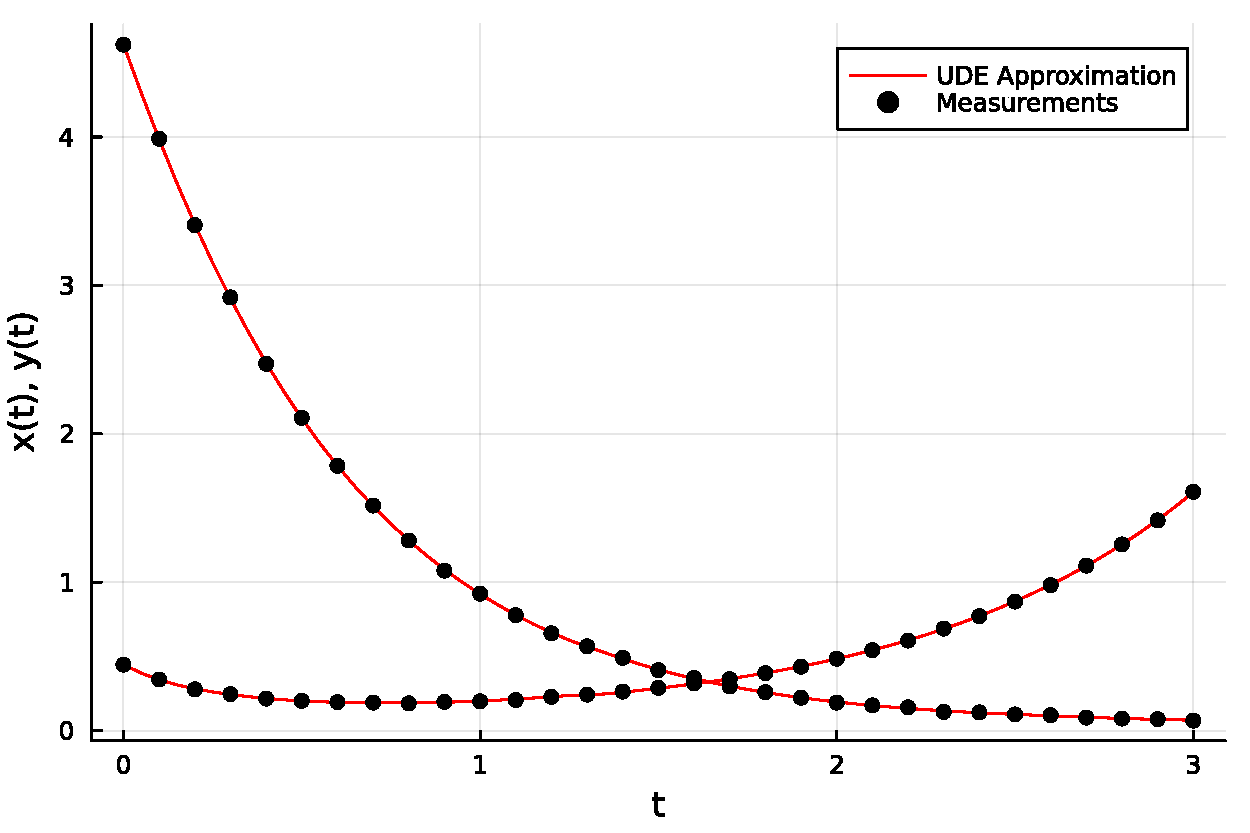
\includegraphics[width=12cm]{plots/Ideal_Data__trajectory_reconstruction.pdf}
\end{frame}

\begin{frame}
  \frametitle{Interaction Reconstruction}
  \begin{itemize}
    \item Neural network approximation vs. true interaction.
  \end{itemize}
  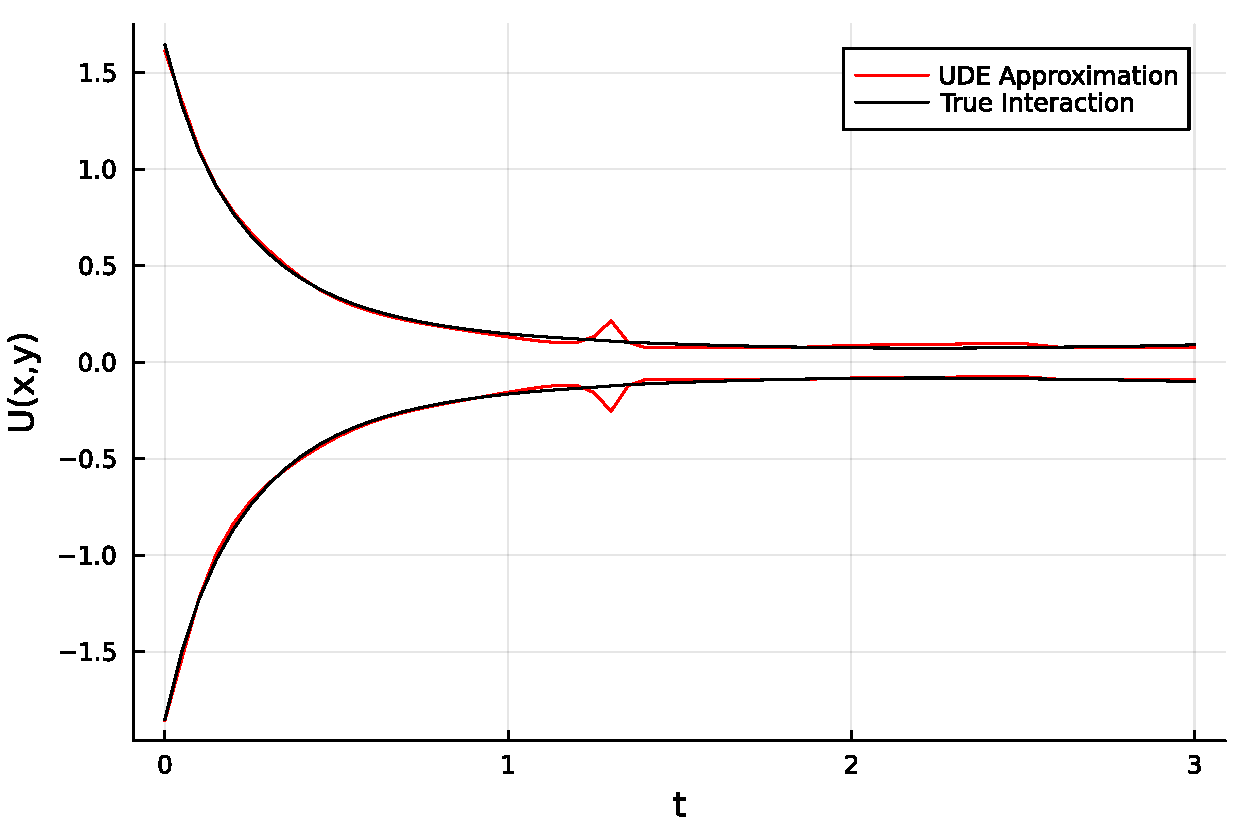
\includegraphics[width=12cm]{plots/Ideal_Data__missingterm_reconstruction.pdf}
\end{frame}

\begin{frame}
  \frametitle{Prediction and Error}
  \begin{itemize}
    \item Error analysis between true interaction and neural network guess.
  \end{itemize}
  \begin{center}
        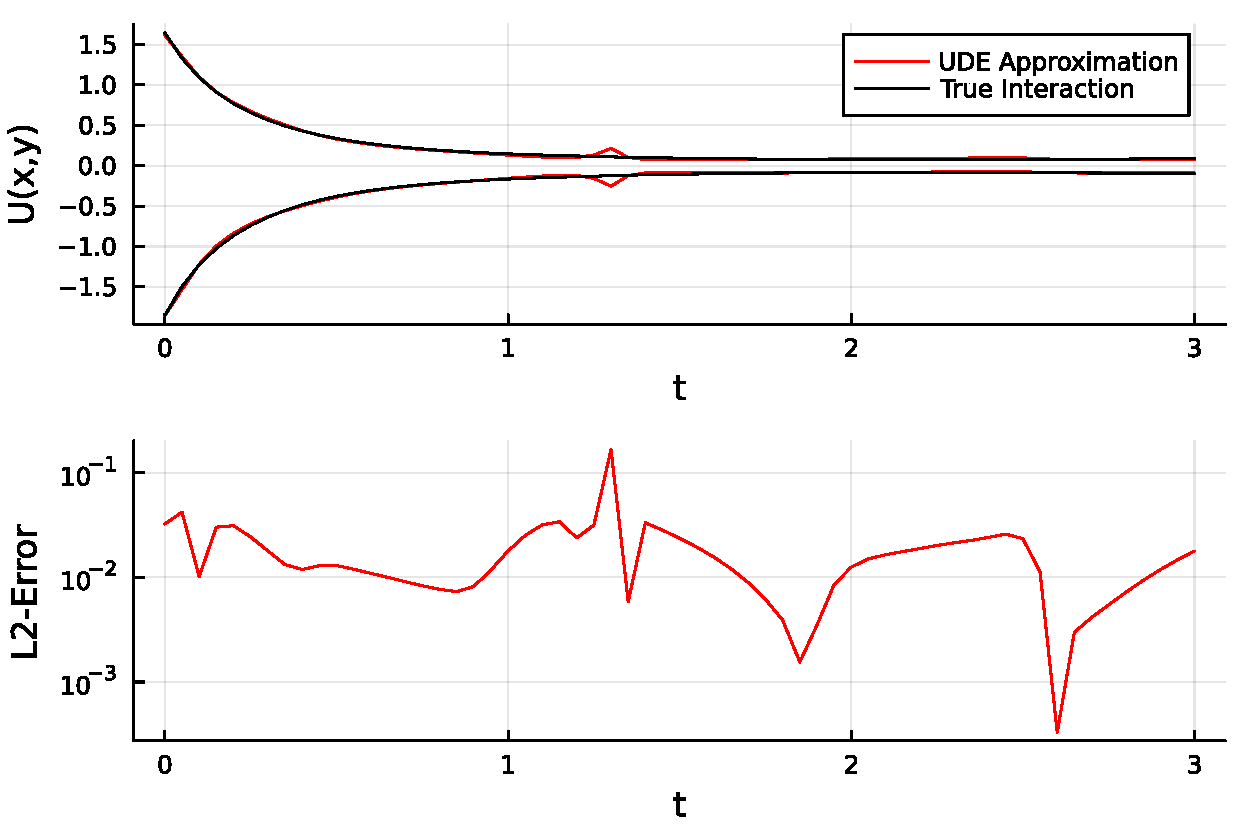
\includegraphics[width=9cm, height=6cm]{plots/Ideal_Data__missingterm_reconstruction_and_error.pdf}
  \end{center}
\end{frame}

\begin{frame}
  \frametitle{Standard Lotka-Volterra Model}
  \begin{itemize}
    \item Extended predictions over 50 time periods.
  \end{itemize}
  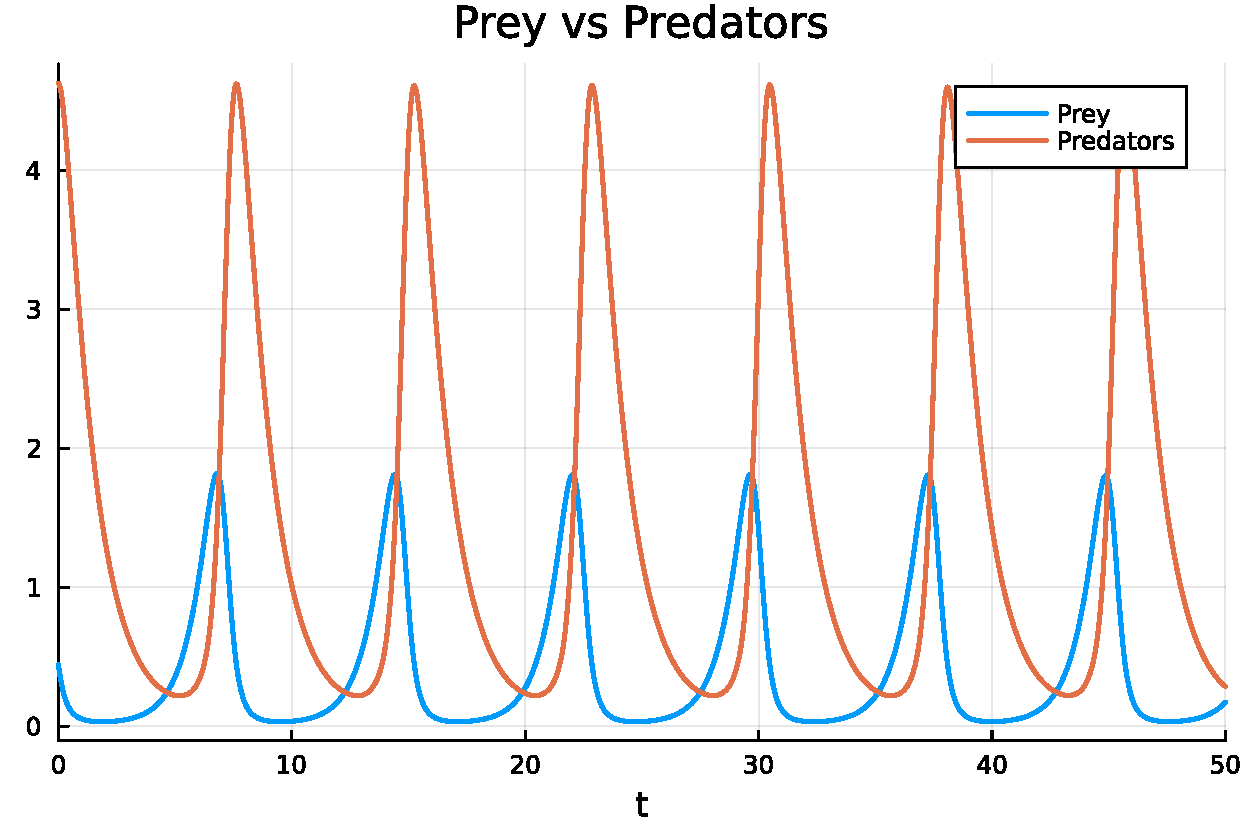
\includegraphics[width=12cm]{plots/algae_vs_predators.pdf}
\end{frame}

\begin{frame}
  \frametitle{Node Model Data Extrapolation}
  \begin{itemize}
    \item Extended predictions over 20 time periods.
  \end{itemize}
  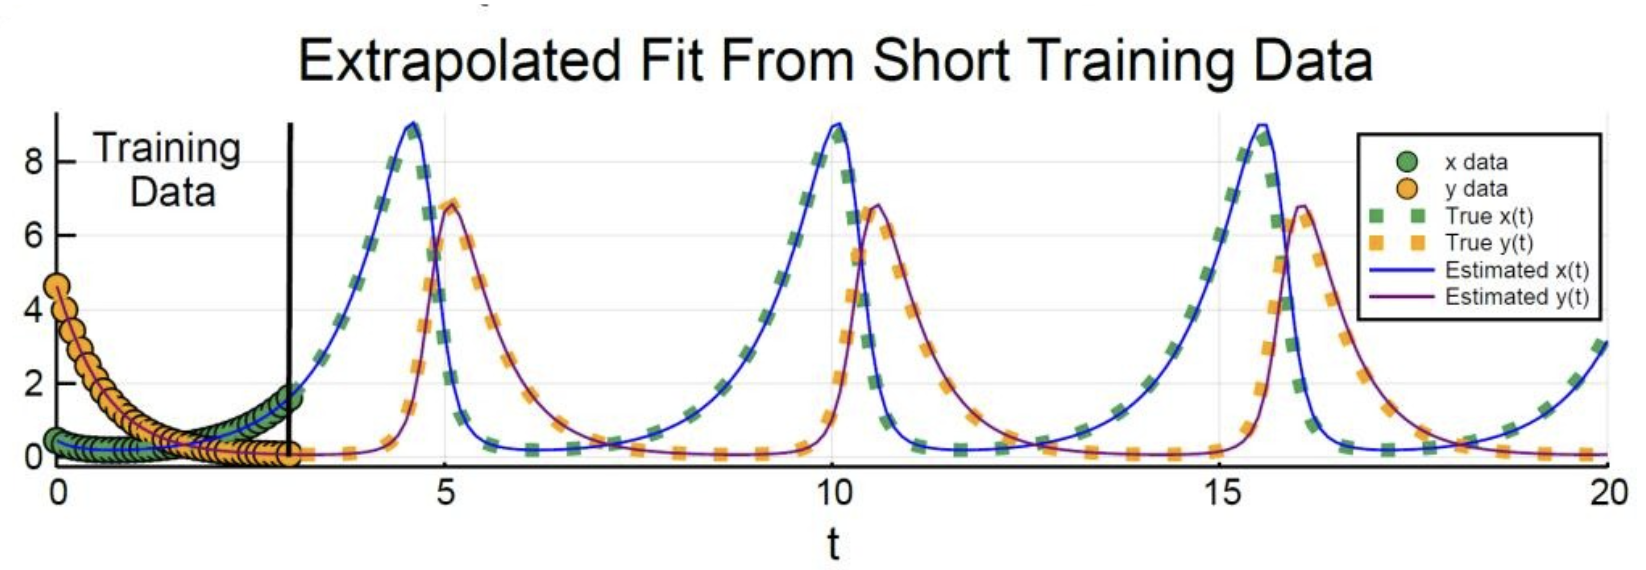
\includegraphics[width=12cm]{plots/Extrapolated_fit.png}
\end{frame}

\begin{frame}
  \frametitle{Application to Real Data}
  \begin{itemize}
    \item Experimental Predator-Prey data between Planktonic Rotifers and Unicellular Algae in a Chemostat.
  \end{itemize}
  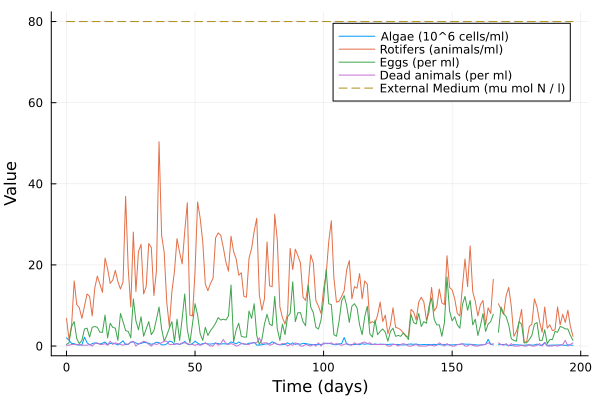
\includegraphics[width=10cm, height = 6.66cm]{plots/output_plot.png}
\end{frame}

\begin{frame}
  \frametitle{Application to Real Data(cont.)}
  \begin{itemize}
  \end{itemize}
  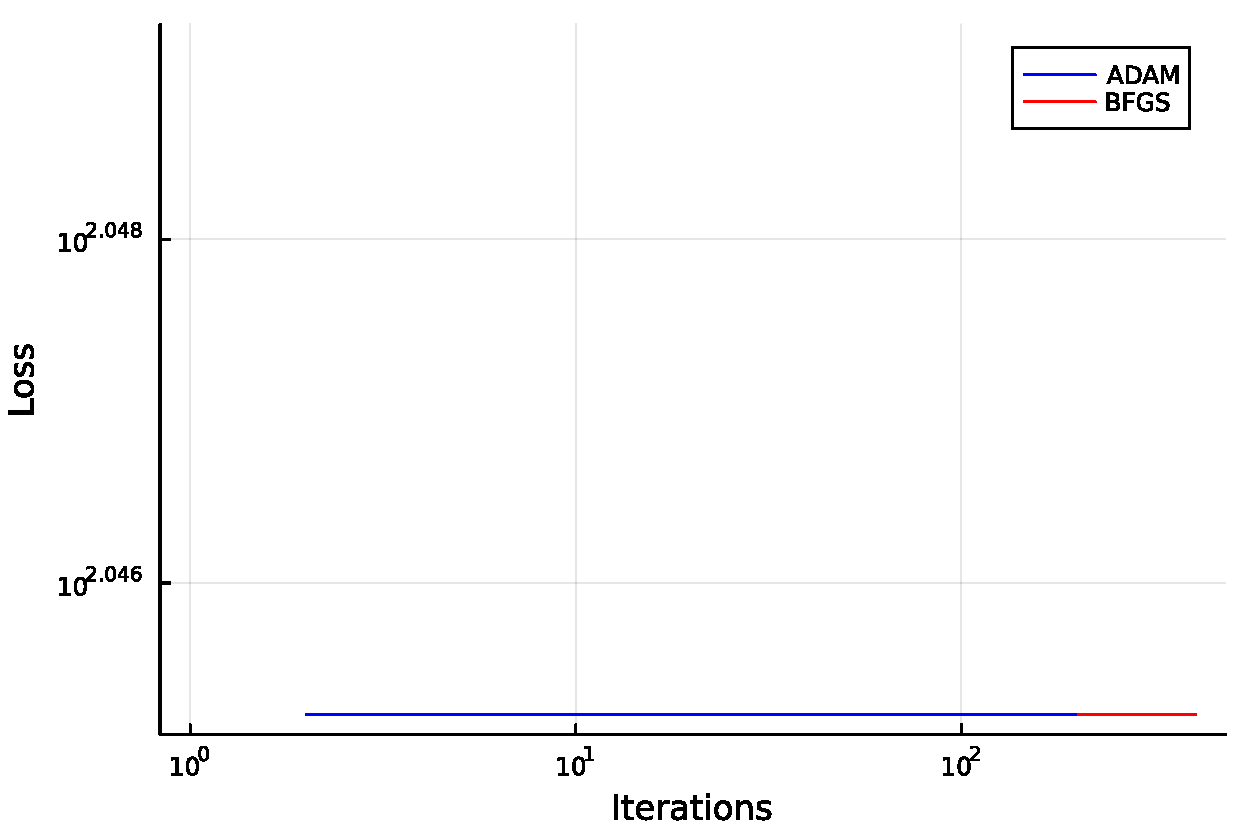
\includegraphics[width=12cm]{plots/Chemostat_losses.pdf}
\end{frame}

\begin{frame}
  \frametitle{Implications for Future Research}
  \begin{itemize}
    \item Integration of larger neural networks.
    \item Application to other ODE systems.
  \end{itemize}
\end{frame}

\end{document}
